\documentclass[11pt]{article}
\usepackage{hyperref}
\usepackage{graphicx}
\usepackage{caption}
\usepackage{geometry}
\usepackage{float}
\usepackage{amsmath}
\usepackage{algorithm}
\usepackage{algpseudocode}
\usepackage{tikz}
\usepackage{enumitem}
\usepackage{tabularx}
\usepackage{makecell}
\usepackage{biblatex}
\usepackage{appendix}
\usepackage{subcaption}
\usepackage{listings}
\usepackage{wrapfig}
\usepackage{ragged2e}

\addbibresource{bibliography.bib}

\geometry{a4paper, margin=1.5cm}
\setlength{\parindent}{0em}
\setlength{\parskip}{0.5em}

\begin{document}

\begin{titlepage}
    \centering
    \vspace*{3cm}
    {\Huge\bfseries Deliverable exercise FC: Compound Pendulum\par}
    \vspace{1cm}
    {\large Mauro VÁZQUEZ CHAS, Dániel MÁCSAI \par}
    \vspace{4cm}
    {\large \textbf{Master in Artificial Intelligence}\par}
    
\includegraphics[width=0.5\textwidth]{Logo_UPC.png}\par\vspace{1cm}
    {\large \textbf{Planning and Approximate Reasoning}\\ Work 4\par}
    \vspace{1cm}
    {\large\bfseries 10th January 2024\par}
\end{titlepage}

\pagestyle{empty}

\newpage
\tableofcontents
\newpage

% Set page numbering    
\setcounter{page}{1}
\pagestyle{plain}

\section{Introduction}
\label{sec:introduction}

\section{Design of the Fuzzy Controller}
\label{sec:desig}

\subsection{Membership functions}
- Error: 

- Error Derivative: 
TODO comment on how we changed the error derivative to [-15 15] from [-5 5]
Reason: it was out of bounds, and the fuzzy controller returned 0 in the Simulink simulation

- Thrust: 

Maybe comment about that defining the lowest (and highest) membership function as a triangle (which decreases after reaching its maximum, if we further decrease it: see screenshot) is not a good idea in our opinion as it is not realistic, but we did it this way to follow the instructions since, it was defined as a triangle in the exercise.

\subsection{Rules}

\begin{table}[h!]
    \centering
    \begin{tabular}{@{}>{\raggedright\arraybackslash}p{12cm}c@{}}
    \toprule
    \textbf{Rule} & \textbf{Weight} \\ \midrule
    If Error is Negative and ErrorDerivative is Decreasing then Thrust is Negative & 1 \\
    If Error is Zero and ErrorDerivative is Decreasing then Thrust is Negative & 1 \\
    If Error is Positive and ErrorDerivative is Decreasing then Thrust is Positive & 1 \\
    If Error is Negative and ErrorDerivative is Stationary then Thrust is Negative & 1 \\
    If Error is Zero and ErrorDerivative is Stationary then Thrust is Zero & 1 \\
    If Error is Positive and ErrorDerivative is Stationary then Thrust is Positive & 1 \\
    If Error is Negative and ErrorDerivative is Increasing then Thrust is Negative & 1 \\
    If Error is Zero and ErrorDerivative is Increasing then Thrust is Positive & 1 \\
    If Error is Positive and ErrorDerivative is Increasing then Thrust is Positive & 1 \\ \bottomrule
    \end{tabular}
    \caption{Rules and Corresponding Weights}
    \label{tab:rules}
    \end{table}
    

\section{Results}

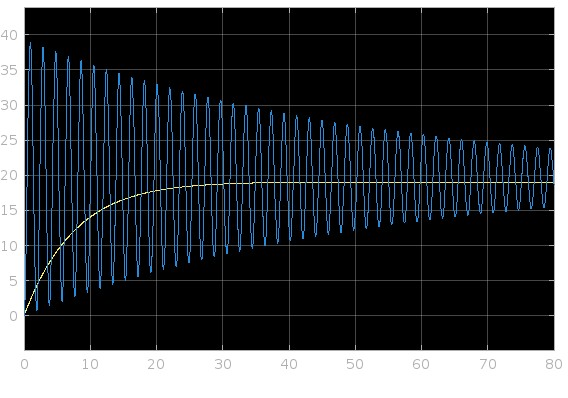
\includegraphics[width=0.6\textwidth]{simulation1.jpg}\par\vspace{1cm}
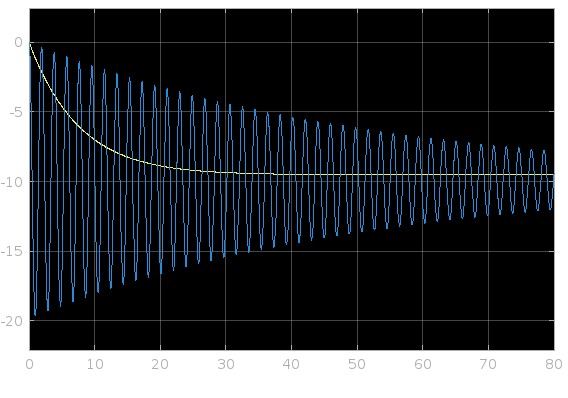
\includegraphics[width=0.6\textwidth]{simulation2.jpg}\par\vspace{1cm}

\section{More complex controller}

(with at least 7 membership functions)

TODO: "Explain and reason what happens if you increase the number of membership functions (7 or more) 
of the output?"

It doesnt talk about it, but if we design the 7 membership functions and the rules, we can implement it in another controller, and run the simulation to see what happens.
I've created pendulum-fuzzy-complex.fis, but so far it is the copy of the original, nothing is modified. 


\section{Conclusions}

%------------------------------------------------------------------------------------------------------------------------------
\section*{References}
\printbibliography[heading=none]

\end{document}